%
% Firewall
%
% Aleph Objects Firewall
%
% Copyright (C) 2014, 2015, 2016 Aleph Objects, Inc.
%
% This document is licensed under the Creative Commons Attribution 4.0
% International Public License (CC BY-SA 4.0) by Aleph Objects, Inc.
%
\begin{figure}[h!]
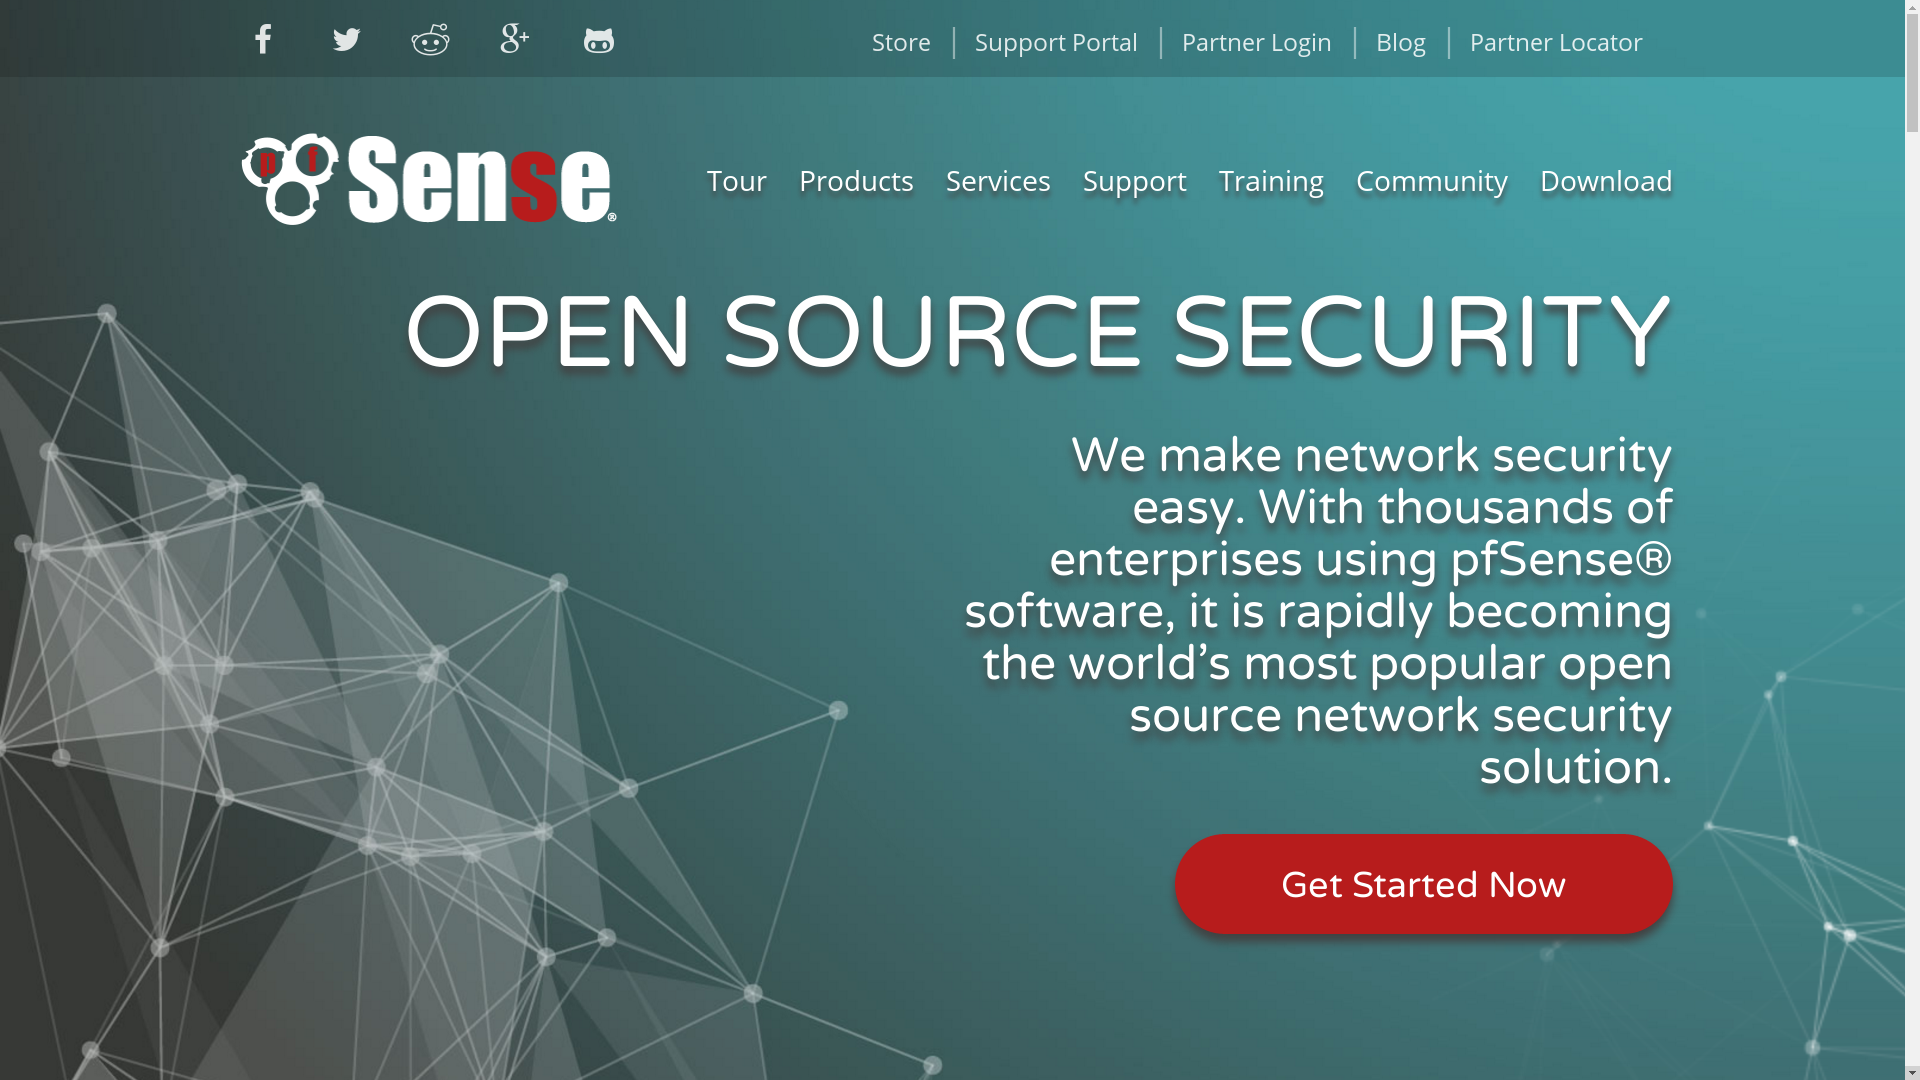
\includegraphics[keepaspectratio=true,height=1.10\textheight,width=1.00\textwidth,angle=0]{www-pfsense.png}
 \caption{pfSense Website}
 \label{fig:www-pfsense}
\end{figure}

\section{Overview}
Aleph Objects has recently deployed pfSense firewalls, replacing OpenBSD.
Most servers and workstations run GNU/Linux, which uses iptables.

\href{https://www.pfsense.org/}{pfSense} --- ``Free, open source customized
distribution of FreeBSD specifically tailored for use as a firewall and router
that is entirely managed via web interface.''

pfSense was selected as Aleph Objects core router/firewall for backbone
connections.

\section{Initial Configuration Overview}

These are the the initial configuration steps for a pfSense firewall. Here is an overview of the steps:

\begin{enumerate}
 \item Make serial connection to pfSense firewall, and do basic initial setup.
 \item Connect to pfSense firewall via web browser.
 \item Do more initial setup.
 \item Connect pfSense router to Internet.
 \item Update router.
 \item Install new packages.
 \item Configure packages.
 \item Backup \& reboot.
\end{enumerate}

\subsection{Setup via Serial Connection}

\begin{enumerate}
 \item Plug the pfSense provided USB cable into the Console port on the firewall and the USB port of your Debian workstation.
 \item Find where the USB device connected, by running \mintinline{sh}{dmesg -T} on your Debian workstation.
Look for a line with USB0, USB1, etc. in it, such as:
\begin{minted}{sh}
usb 1-6: cp210x converter now attached to ttyUSB0
\end{minted}
 \item Run \texttt{minicom} on your workstation to connect to the router, using the USB device from above.
\begin{minted}{sh}
sudo minicom -D /dev/ttyUSB0
\end{minted}



 \item 115200 baud, 8N1, no flow control.
 \item Copy MAC address to main DHCP/DNS server, and reserve IP address.
 \item Set IP for LAN (e.g. 192.168.1.1)
 \item Set IP for WAN, disable IPv6
\end{enumerate}

\subsection{Initial Wizard Setup via Web Browser}

\begin{enumerate}
 \item Log in to firewall (e.g. https://192.168.1.1).
       Initial pass admin/pfsense.
 \item Start Wizard, hit Next.
 \item pfSense Gold, Next.
 \item Hostname: set hostname.
 \item Set WAN, LAN, password, etc.
 \item Hit Reload, and the wizard is done.
\end{enumerate}

\subsection{Basic Setup via Web Browser}

\begin{enumerate}
 \item System --> User Manager. Click Add. Add Username, Password, Full name, Experation date leave blank. Move to add to Group membership ``admins'' (presuming this is an admin). Add ssh key, if you want to ssh in. Certificate, leave blank for now (can be used for OpenVPN/RADIUS). 
 \item Log out and log back in as newly created user.
 \item Goto System --> Advanced. Under Admin Access. Set TCP port to randomish port between 1 and 65535. This will be the new pfSense web interface port address. Max processes: 16 (2 is too low, not sure what is ideal). Check WebGUI redirect to disable port 80. Check enable Secure Shell Server. Disable password login. Pick randomish port for SSH. Check to password protect Console menu. Save.
 \item At this point, you can optionally SSH into the firewall if a key was set up for the user.
 \item Under System --> Advanced, Networking. Uncheck Allow IPv6, to disable IPv6 (yay!). Check boxes for: Hardware Checksum Offloading, Hardware TCP Segmentation Offloading, Hardware Large Receive Offloading. These need to be disabled because/if Suricata is used in Inline mode. If it isn't, these can be unchecked and if the hardware is good/can handle it, it will likely be faster. (Side note, enabling Hardware Checksum Offloading breaks networking in a KVM.) Save.
 \item System --> Advanced, Miscellaneous. Cryptographic Hardware should be set to AES-NI for any hardware from pfSense. For other hardware, check dmesg. Thermal Sensors: Intel Core* CPU on-die thermal sensor. Hard disk standby time, 6 minutes (not sure this really has any effect). Host UUID, check Do NOT send HOST UUID with user agent. Save.
 \item System --> Notifications. Check for Disable Growl Notifications and Disable SMTP. Save.
\end{enumerate}

\subsection{SSL Certificate Manager Setup}
\begin{enumerate}
 \item System --> Cert. Manager. Under Certificates, click Add. Method: Create a Certificate Signing Request. Descriptive Name, use the hostname of the firewall being setup. Key length 4096, Digest Algorithm sha512. Country Code US, etc. Common name, use hostname of firewall. Save.
 \item System --> Cert. Manager, Under Certificates, the new cert added above, click Export Request mini-icon. Gandi: Standard SSL, single address, 3 year. Paste in the CSR exported from the mini-icon into Gandi. Select Apache/ModSSL for Software used in Gandi, and if it says the correct ``Main domain (CN)'', hit Submit in Gandi. Delete any .req file that was downloaded by browser. Gandi: Validation by email (probably). It will take ~10+ minutes to get verification back from Gandi (not instant).
 \item System --> Cert. Manager, Under Certificates. When cert is ready and confirmed at Gandi, hit Get the Certificate. Hit the ``Update CSR'' pencil on the appropriate certificate line. Paste the Gandi cert into Final certificate data. Delete any downloaded copies.
 \item System --> Cert. Manager. Under CAs, click Add. Method: Import an existing Certificate Authority. Descriptive Name: ``GandiStandardSSLCA2''. Get the cert from \url{https://www.gandi.net/static/CAs/GandiStandardSSLCA2.pem} and paste into Certificate data. Certificate Private Key, blank. Save. Note, this has to be done after the above Gandi certificate is added to the firewall.
 \item System --> Cert. Manager, also import any of our own CAs and Certificate Revocations, if any.
\end{enumerate}

\subsection{General Setup}
\begin{enumerate}
 \item System --> General Setup. Check all looks good. Top Navigation: Fixed (Remains visible at top of page). Hostname in Menu: Hostname only. (DNS servers can be bound to particular interfaces here, if needed in multi-WAN). Save.
 \item To use the newly set up certifcate. System --> Advanced, Admin Acess. Change SSL Certificate to the new one. Save. Now go to that new hostname with https and the correct port.
\end{enumerate}

\subsection{Initial Firewall Rules}
\begin{enumerate}
 \item Firewall --> Rules. LAN interface, click the pencil to edit the IPv6 line. Change Action to Reject. Change Source to any. Change Description to ``Default Reject LAN IPv6''. Save. Apply Changes.
 \item Firewall --> Rules. Under LAN interface, click the Copy mini-icon to copy the IPv6 line. Change Action to Block. Interface to WAN. Change Description to ``Default Block WAN IPv6''. Save. Apply Changes.
\end{enumerate}

\subsection{Initial DNS Resolver Setup}
\begin{enumerate}
 \item Services --> DNS Resolver. Enable (default). Network Interfaces: just select LAN and localhost. Outgoing Network Interfaces: WAN, LAN, localhost. Add checks for DHCP Registration, Static DHCP. Save. Apply Changes.
 \item Services --> DNS Resolver, Advanced Settings. Add checks for: Prefetch Support, Prefetch DNS Key Support. Increase Message Cache Size to 50 MB or so (?). Save. Apply Changes.
 \item Services --> Dynamic DNS. Setup, if needed.
\end{enumerate}

\subsection{Initial Logging Setup}
Setup logging to the local firewall. Remote logging will be set up.

\begin{enumerate}
 \item Status --> System Logs, Settings. Add checks to Forward/Reverse Display. GUI Log Entries, increase to 200. Where to show rule descriptions ``Display as second row''. This is where remote logging will be set up... 
 \item Status --> Dashboard. Click the Plus + in the upper right corner. Add the available widgets: Gateways, Thermal Sensors, Traffic Graphs, S.M.A.R.T. Status, Firewall Logs, Interface Statistics, OpenVPN, Services Status, NTP Status.
\end{enumerate}

\subsection{Backup}
Make first backup.

\begin{enumerate}
 \item Diagnostics --> Backup \& Restore. Backup.
 \item Diagnostics --> Reboot and make sure everything comes up clean.
\end{enumerate}

\subsection{Internet Connection}
Make initial connection to the Internet with the new pfSense firewall.


At this point, this presumes the WAN interface isn't up and routing actual Internet traffic. It is better to get the router as configured as possible before actually using the WAN interface. Assuming the firewall is on the LAN and being configured, it can use the gateway that is on its LAN interface. When configuration is finalized and the router is deployed, the WAN interface will carry Internet traffic. To to this, add a route by: Interfaces --> LAN. Under IPv4 Upstream gateway, click Add a new gateway. Add the LAN gateway info, and check is as Default gateway (3000). Save. Apply Changes..

\begin{enumerate}
 \item System --> Routing. Click to edit the mini pencil icon on the Gateway line listed as Default. Monitor IP: something appropriate upstream, can use 8.8.8.8. Note: on high latency connections such as satellite, hit Display Advanced and increase Latency thresholds (750, 2500), Packet Loss thresholds (15, 25), Probe Interval (1000), Loss Interval (3000). Save. Apply Changes.
\end{enumerate}

\subsection{Update \& Install Packages}
\begin{enumerate}
 \item System --> Update, System Update. Check that the Status is ``Up to date.'' If it needs updating, update.
 \item System --> Package Manager, Installed Packages. The first time here, you need to click on Available Packages (presumably to download latest package header info). Then go back to Installed Packages. If there are any Installed Packages that have a Newer version available, click the mini icon to update the package. Confirm.
 \item System --> Package Manager, Available Packages. Install: Cron, ntopng, openvpn-client-export, pfBlockerNG, RRD\_Summary, Status\_Traffic\_Totals, sudo, suricata.
 \item System --> sudo. Add user, optionally.
\end{enumerate}


\subsection{OpenVPN}
OpenVPN is run by a collection of pfSense firewalls.

\begin{enumerate}
 \item OpenVPN setup.
 \item System --> Cert. Manager. Set up internal certificate authority.
 \item System --> Cert. Manager. Create internal server certificate.
 \item SSH into firewall. pfSense ships with pre-generated DH keys, due to ``heavy computation''. This can take an hour for 4096.
\begin{minted}{sh}
/usr/bin/openssl dhparam 1024 > /etc/dh-parameters.1024
/usr/bin/openssl dhparam 2048 > /etc/dh-parameters.2048
/usr/bin/openssl dhparam 4096 > /etc/dh-parameters.4096
\end{minted}
 \item VPN --> OpenVPN. Set up VPN server. Server Mode: Remote Access (SSL/TLS + User Auth). Backend for Authentication: Local Database (will be FreeRADIUS at some point). Protocol: UDP. Local Port: something randomish. Peer Certificate Authority: use the interal CA created earlier. Server Certificate: Use the server certificate created earlier. DH Parameter length (bits): 4096. Encryption Algorithm: AES-256-CBC (256-bit), this has hardware crypto support on pfSense routers. Auth digest algorithm: SHA512 (512-bit). Hardware Crypto: BSD Cryptodev engine- RSA, DSA, DH, AES-128-CBC, AES-192-CBC, AES-256-CBC. Certificate Depth: One. Strict User-CN Matching: check Enforce Match once it is confirmed working. IPv4 Tunnel Network: Set the new VPN network. IPv6 Tunnel Network: leave blank. Redirect Gateway: unchecked.  IPv4 Local network(s): set the local LAN network. IPv6 Local network(s): leave blank. Compression: Enabled with Adaptive Compression. Inter-client communication: Checked. Disable IPv6: Checked. Dynamic IP: Unchecked, at least for now. Topology: subnet. DNS Default Domain: Checked, and set domain. DNS Server enable: Checked. DNS Server 1: enter servers. Save.
 \item System --> User Manager. Add user for VPN. Certificate: Check to create user certificate. Descriptive name: username.domainname. Certificate Authority: Select internal CA created above. Key length: 4096. Lifetime: 1095.
 \item VPN --> OpenVPN, Client Export. Remote Access Server: Select the VPN server created earlier. Verify Server CN: automatic. Block Outside DNS: Checked. At the bottom, export as Standard Configurations, Archive to use with another pfSense server. To use with OpenVPN in F-Droid (Android), use Inline Configurations (Android).
\end{enumerate}


\subsection{Turn off Internet via LAN}
\begin{enumerate}
 \item Interfaces --> LAN. When you're done using the LAN as any sort of gateway. Change IPv4 Upstream gateway to None. Save. Apply Changes.
\end{enumerate}

\subsection{More Backup}
Make another backup.

\begin{enumerate}
 \item Diagnostics --> Backup \& Restore. Backup.
 \item Diagnostics --> Reboot and make sure everything comes up clean.
\end{enumerate}


\section{NAT}
Network Address Translation.

\begin{itemize}
 \item VoIP using SIP is often a problem behind a NAT.
 \item Enable Keepalives in Grandstream phones to connect to the Asterisk server.
 \item Disable ALG (Application Level Gateway) in any consumer/home routers.
\end{itemize}


\section{Traffic Shaping}
\begin{itemize}
 \item Prioritize admin ssh to firewalls/servers (in case of DoS, etc.)
 \item Prioritize VoIP
 \item De-prioritize SMTP, etc...
\end{itemize}

\section{pfBlockerNG}
\begin{itemize}
 \item IP blocklists for botnets, etc.
\end{itemize}


\section{Suricata}
Suricata is being used as an Intrusion Detection System.
It is preferred over Snort as Suricata is multithreaded and Snort isn't.

\begin{figure}[h!]
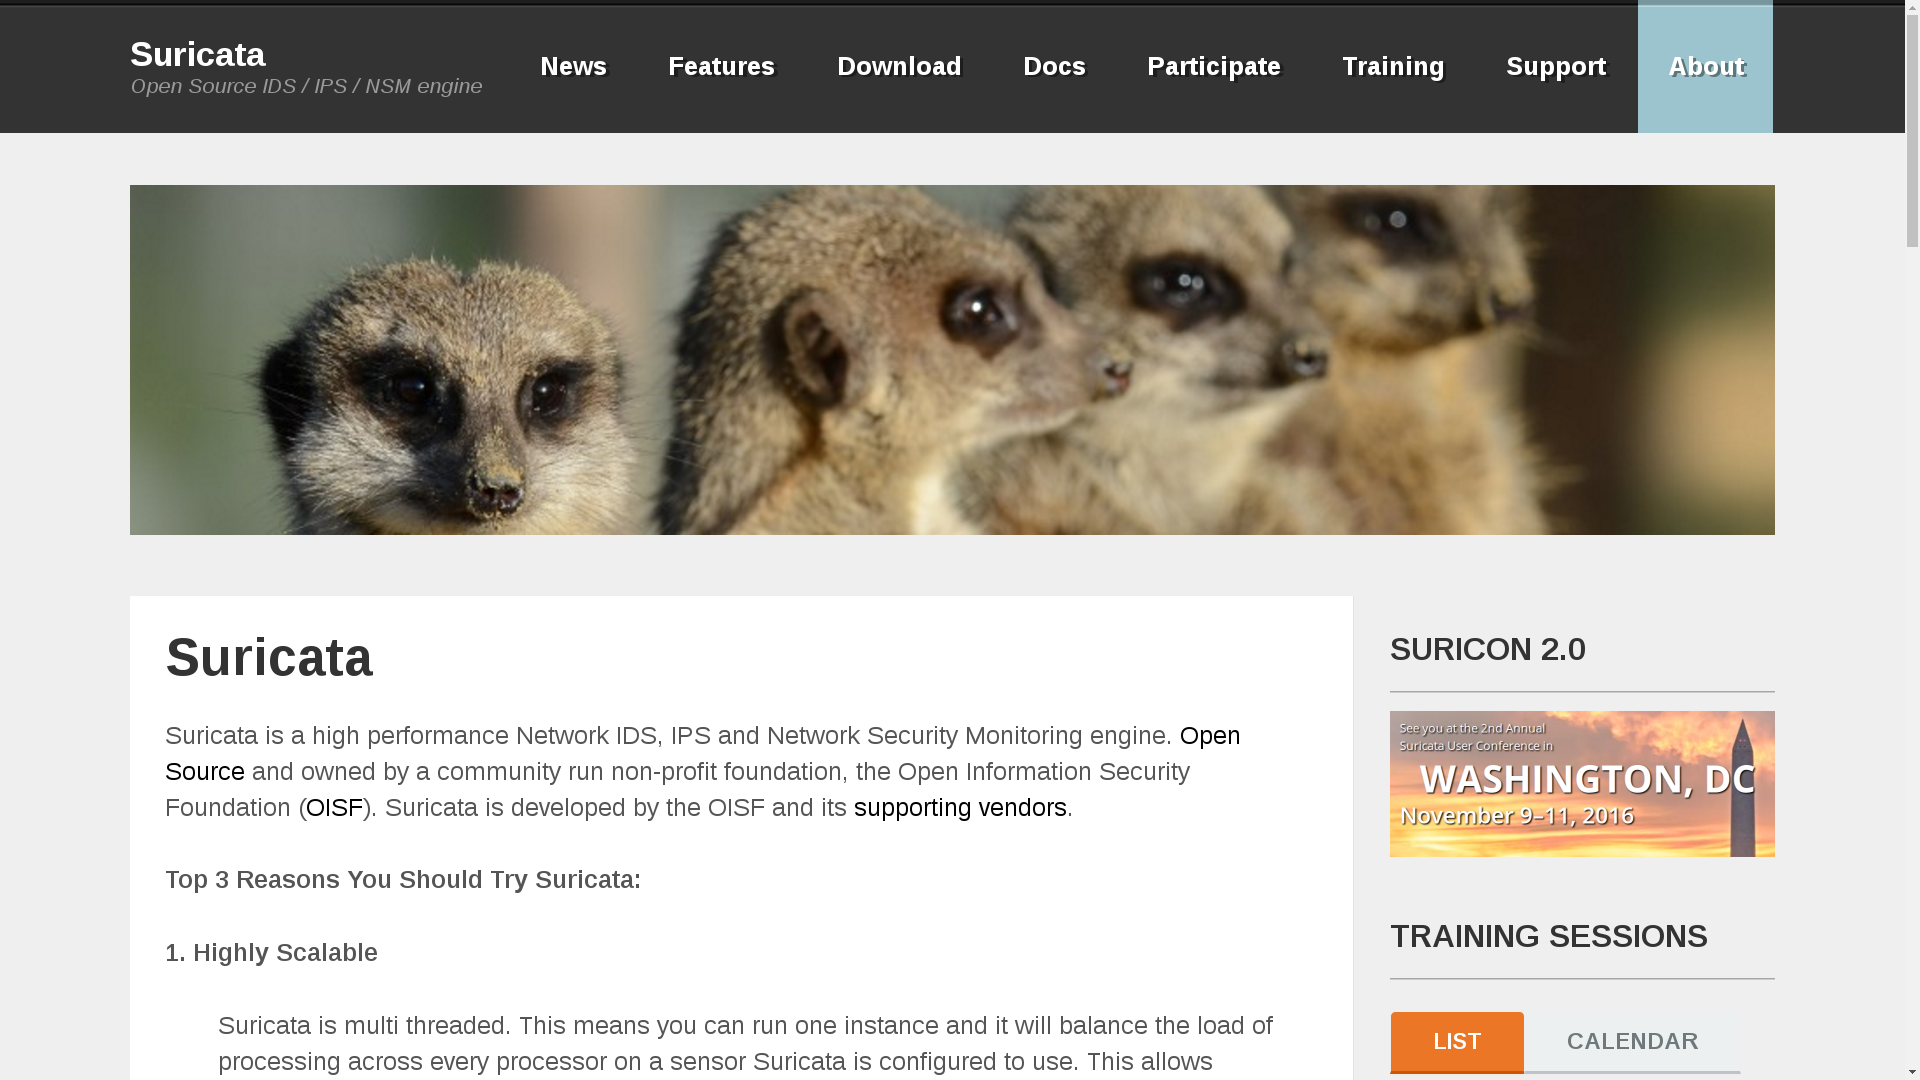
\includegraphics[keepaspectratio=true,height=1.10\textheight,width=1.00\textwidth,angle=0]{www-suricata.png}
 \caption{Suricata Website}
 \label{fig:www-suricata}
\end{figure}

\begin{itemize}
 \item barnyard2
 \item Snort Blacklists
 \item Emerging Threats Blacklists
 \item GeoIP
 \item Alerts, Blocks, Suppress
 \item SID
\end{itemize}


\section{DHCP}
For DHCP services, pfSense uses Dnsmasq, which is also used for DNS
forwarding.


%Services --> DHCP Server. Note: for netboot install of a workstation. Set up DHCP address. Network Booting, show advanced. Enable network booting for that host. Set Next Server to the IP address of the tftp server. Set XXX to ``jessie_crypto'' for encrypted install or ``jessie'' for a regular install.
\begin{enumerate}
 \item Services --> DHCP Server. Network Booting, click Display Advanced. Check box for Enables Network Booting. Set Default BIOS file name to jessie\_crypto/pxelinux.0 or jessie/pxelinux.0. Set Next Server to IP address of tftp server. Save.
 \item Services --> DHCP Server. Go to the bottom and hit Add. Add the MAC address, Client Identifier (hostname), IP Address, Hostname, Netboot Filename (we probably don't need it in the general config), and TFTP Server.
\end{enumerate}

\begin{itemize}
 \item Disable IPv6.
 \item tftp netboot installs.
 \item Static mappings.
\end{itemize}


\section{NTP}


\section{OpenVPN}
\begin{figure}[h!]
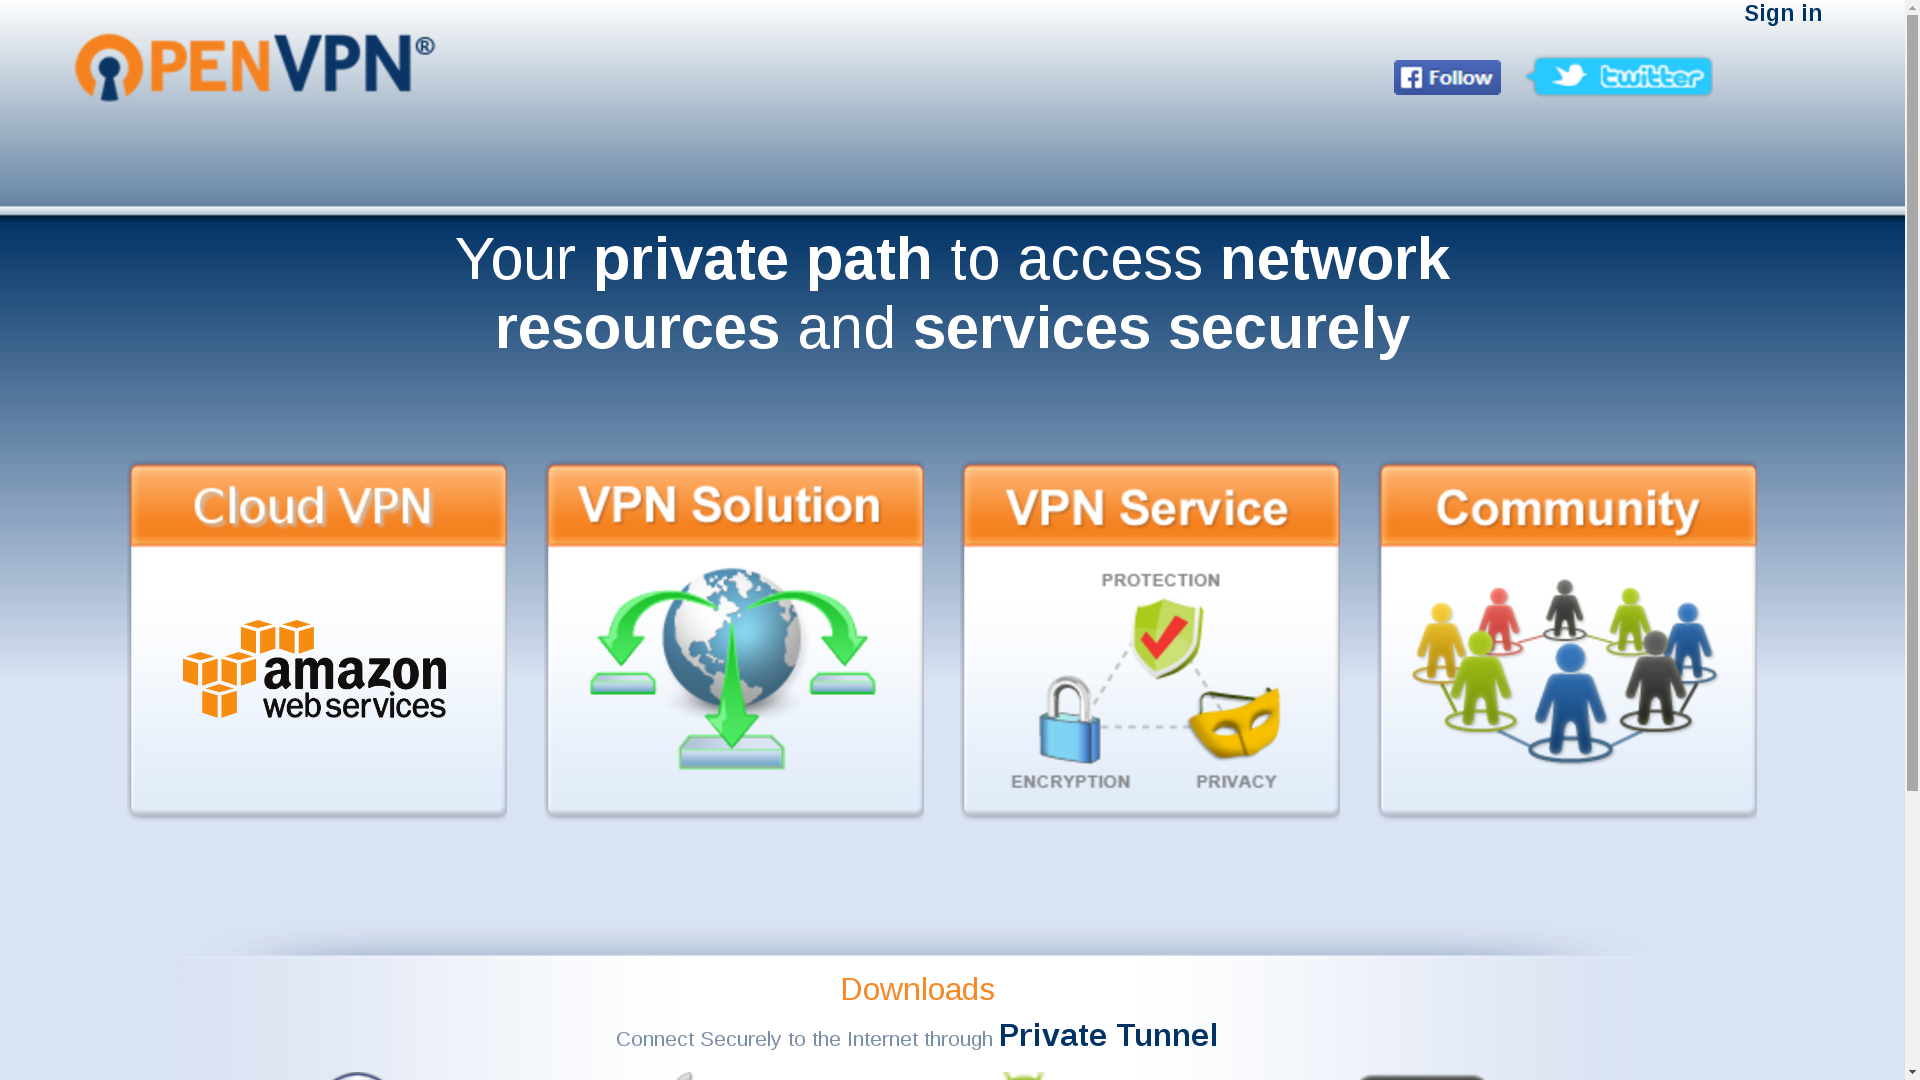
\includegraphics[keepaspectratio=true,height=1.10\textheight,width=1.00\textwidth,angle=0]{www-openvpn.png}
 \caption{OpenVPN Website}
 \label{fig:www-openvpn}
\end{figure}


Virtual Private Networks.


\href{https://www.openvpn.net/}{OpenVPN} --- ``OpenVPN is a full-featured open source SSL VPN solution that accommodates a wide range of configurations, including remote access, site-to-site VPNs, Wi-Fi security, and enterprise-scale remote access solutions with load balancing, failover, and fine-grained access-controls.''

\begin{itemize}
 \item Network design (e.g. many point to point, one central server, etc.).
 \item Main OpenVPN server.
 \item Other internal servers.
 \item External servers private connections.
 \item Laptops.
 \item Mobiles.
 \item SSL certificates.
 \item AES-256-CBC is hardware accelerated on pfSense routers.
 \item SHA512 Auth digest algorithm
 \item Hardware Crypto: BSD cryptodev engine
\end{itemize}


pfSense ships with pre-generated DH keys, due to ``heavy computation''.
This can take an hour for 4096.
\begin{minted}{sh}
/usr/bin/openssl dhparam 1024 > /etc/dh-parameters.1024
/usr/bin/openssl dhparam 2048 > /etc/dh-parameters.2048
/usr/bin/openssl dhparam 4096 > /etc/dh-parameters.4096
\end{minted}



\section{Captive Portal}
The Captive Portal for Aleph Mountain building wifi services.


\section{SSL Certificates}
pfSense makes it very easy to generate Certificate Signing Requests (CSRs),
which can be send to Gandi.net to get issued a ``properly'' signed SSL
certificate.


\section{ssh}
OpenSSH from OpenBSD is used. The BSD shell is a bit different from GNU.


\section{DNS}
DNS forwarding is provided by Dnsmasq.

\begin{figure}[h!]
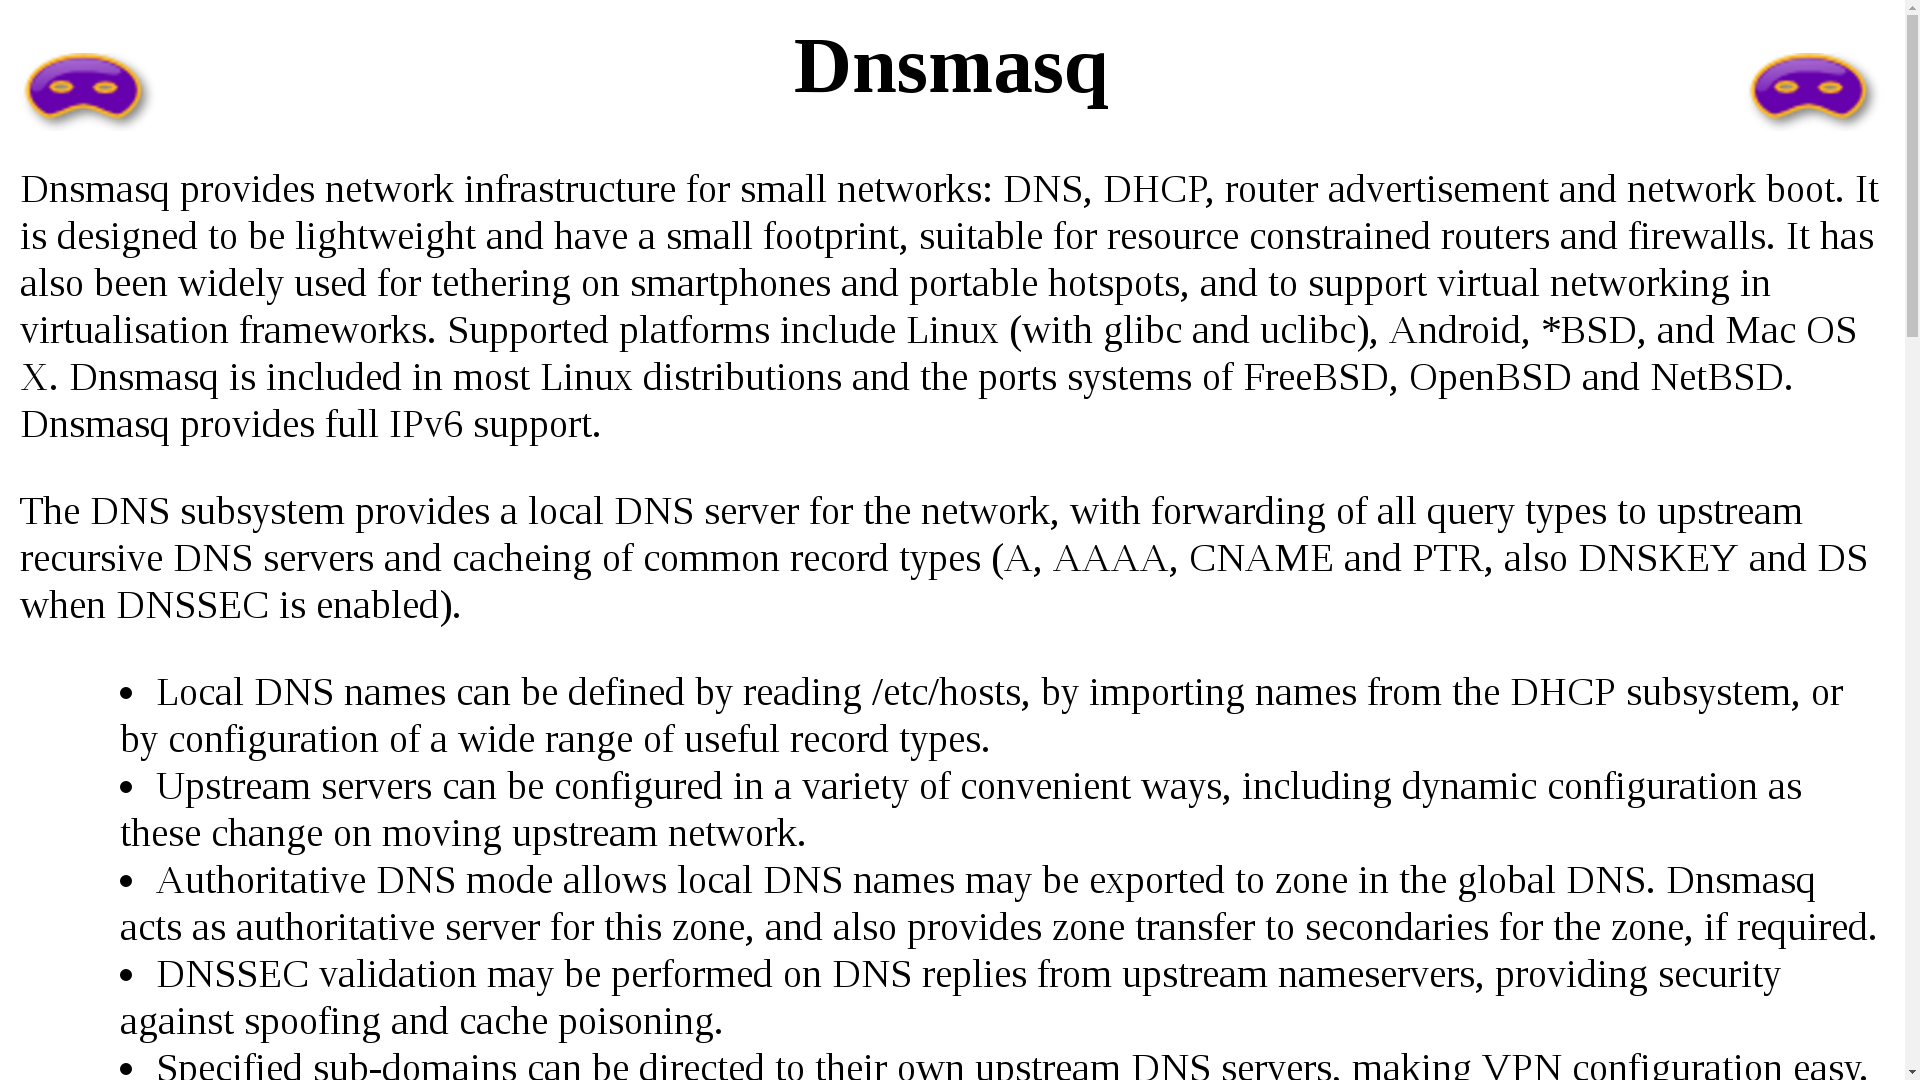
\includegraphics[keepaspectratio=true,height=1.10\textheight,width=1.00\textwidth,angle=0]{www-dnsmasq.png}
 \caption{Dnsmasq Website}
 \label{fig:www-dnsmasq}
\end{figure}



\section{Routing}
\begin{itemize}
 \item No BGP, OSPF, etc.
 \item Static backbone routes.
 \item WAN failover
\end{itemize}


\section{Interfaces}

\begin{itemize}
 \item Gigabit ethernet.
 \item SFP+.
 \item Hardware offloading (e.g. checksums).
\end{itemize}


\section{CARP and Synchronization}
CARP can be used to have transparent failover to another firewall, if one
firewall on the network should drop.

Synchronization between CARP firewalls allows easy configuration updates. For
instance, if a configuration change is made to the DHCP server, it can
``instantly'' push to the backup firewall.


\section{Reporting}

\begin{figure}[h!]
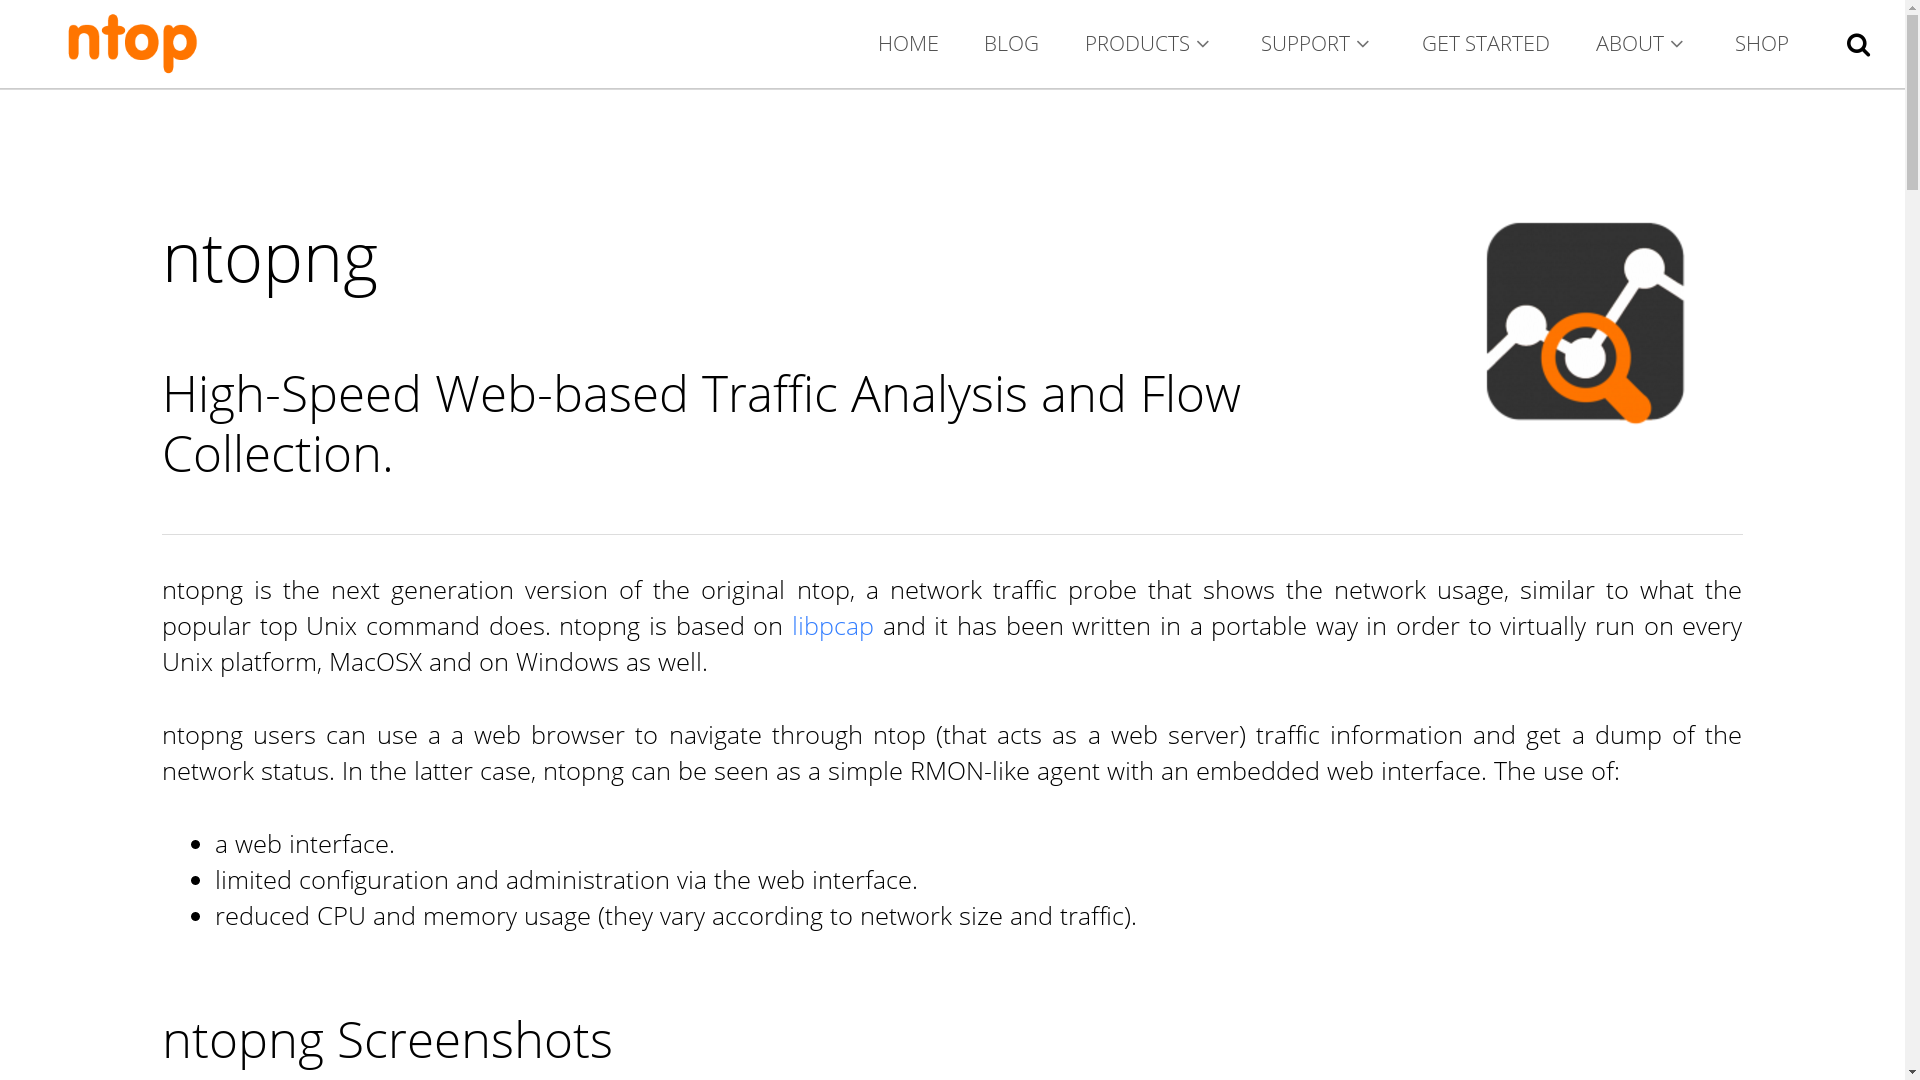
\includegraphics[keepaspectratio=true,height=1.10\textheight,width=1.00\textwidth,angle=0]{www-ntopng.png}
 \caption{ntopng Website}
 \label{fig:www-ntopng}
\end{figure}

\begin{itemize}
 \item Dashboard.
 \item Darkstat.
 \item ntopng (``Network Top Next Generation'' ?).
 \item S.M.A.R.T.
 \item System Temperatures.
 \item MRTG
 \item RRD
\end{itemize}

